%%%% AutoDSC --- IEEE ICDM 2026 (IEEE conference format)
\documentclass[conference]{IEEEtran}
\IEEEoverridecommandlockouts
% The preceding line is only needed to identify funding in the first footnote.
% If unneeded, comment it out.

\usepackage{cite}
\usepackage{amsmath,amssymb,amsfonts}
\usepackage{amsthm}
\usepackage[linesnumbered,ruled,vlined]{algorithm2e}
\usepackage{graphicx}
\usepackage{textcomp}
\usepackage{xcolor}
\usepackage{booktabs}
\usepackage{multirow}
\usepackage{array}
\usepackage[caption=false,font=footnotesize]{subfig} % \subfloat; caption=false avoids the caption-pkg warning
\usepackage{url}
\usepackage[hidelinks]{hyperref}

\def\BibTeX{{\rm B\kern-.05em{\sc i\kern-.025em b}\kern-.08em
    T\kern-.1667em\lower.7ex\hbox{E}\kern-.125emX}}

\begin{document}

\title{AutoDSC: An Automated Data Stream Clustering Framework}

% For double-blind review, comment out the author block below and use the
% anonymous one. The real author block is provided for the camera-ready.
\author{\IEEEauthorblockN{Anonymous}}

% \author{
% \IEEEauthorblockN{Nilesh Verma}
% \IEEEauthorblockA{\textit{AI Institute} \\ \textit{University of Waikato} \\ Hamilton, New Zealand \\ nv78@students.waikato.ac.nz}
% \and
% \IEEEauthorblockN{Albert Bifet}
% \IEEEauthorblockA{\textit{AI Institute} \\ \textit{University of Waikato} \\ Hamilton, New Zealand \\ albert@waikato.ac.nz}
% \and
% \IEEEauthorblockN{Bernhard Pfahringer}
% \IEEEauthorblockA{\textit{AI Institute} \\ \textit{University of Waikato} \\ Hamilton, New Zealand \\ bernhard@waikato.ac.nz}
% \and
% \IEEEauthorblockN{Maroua Bahri}
% \IEEEauthorblockA{\textit{CNRS, LIP6} \\ \textit{Sorbonne Universit\'e} \\ Paris, France \\ maroua.bahri@lip6.fr}
% }

\maketitle

\begin{abstract}
Data stream clustering faces unique challenges in dynamic environments where data distributions evolve continuously and computational resources are limited. While AutoML has transformed supervised learning, its application to unsupervised streaming tasks remains largely unexplored. Traditional clustering algorithms are sensitive to algorithm selection, hyperparameter configuration, and changes in data characteristics. We introduce AutoDSC (Automated Data Stream Clustering), a novel framework that automatically optimizes algorithm selection and hyperparameter tuning for real-time stream clustering. AutoDSC employs Population-Guided Stochastic Search Optimization (PGSSO), leveraging a recency-weighted elite archive to guide efficient parameter exploration while dynamically adjusting the exploration rate based on performance feedback. The framework adapts to concept drift implicitly: every window it re-evaluates the population and re-selects the incumbent, and its exploration rate rises automatically when clustering quality degrades. Robust performance assessment is provided by a multi-objective score combining three clustering validation indices. Our theoretical analysis establishes regret bounds for the optimization process. Across ten real-world and synthetic streams, AutoDSC attains the best mean rank on both the Adjusted Rand Index and CMM and the highest mean ARI among all methods---significantly outperforming untuned single algorithms---while being the most computationally efficient of the automated approaches, processing $2$--$3\times$ more instances per second than competing AutoML stream clusterers at a lower memory footprint.
\end{abstract}

\begin{IEEEkeywords}
data stream clustering, AutoML, concept drift, hyperparameter optimization, online learning
\end{IEEEkeywords}

\section{Introduction}

Automated Machine Learning (AutoML) has significantly advanced the accuracy and efficiency of machine learning workflows by automating tasks such as algorithm selection, hyperparameter optimization, and pipeline synthesis~\cite{hutter2019automated}. While AutoML has seen widespread adoption in supervised learning, its application to clustering remains comparatively less explored, mainly due to the absence of a universally applicable objective function for evaluation~\cite{poulakis2024survey}. Recent AutoML solutions for clustering include AutoML4Clust~\cite{Tschechlov2021AutoML4Clust}, AutoCluster~\cite{Liu2021AutoCluster}, cSmartML~\cite{ElShawi2021cSmartML}, ML2DAC~\cite{TrederTschechlov2023ML2DAC}, TPE-AutoClust~\cite{ElShawi2025TPEAutoClust}, and PoAC~\cite{daSilva2024PoAC}. These approaches address clustering challenges using various automated methodologies such as meta-learning, pipeline composition, and problem-specific heuristics.

However, with the increasing availability of streaming data from sources like Internet of Things (IoT) sensors, web traffic, and social media, traditional static AutoML approaches are insufficient~\cite{yang2022iot}. They cannot adapt to dynamic environments or process data in a single pass due to concept drift and memory limitations~\cite{bifet2018machine}. Existing online AutoML frameworks such as Online AutoML~\cite{celik2023online}, ASML~\cite{pmlr-v256-verma24a}, ChaCha~\cite{pmlr-v139-wu21d}, and Auto-Reg~\cite{verma2025auto-reg} primarily focus on supervised learning tasks. Meanwhile, unsupervised learning, particularly clustering, requires specialized AutoML solutions. At present, ConfStream~\cite{carnein2020confstream} and OnlineAutoClust~\cite{el2023onlineautoclust} represent the only established AutoML solutions for stream clustering. Nevertheless, they suffer from significant limitations. ConfStream relies on single clustering evaluation metrics, and OnlineAutoClust uses computationally intensive offline search methods, which are inefficient for real-time streaming scenarios. These limitations highlight the critical need for tailored AutoML solutions designed specifically for data stream clustering~\cite{bahri2021data}. This paper introduces AutoDSC (Automated Data Stream Clustering), a comprehensive AutoML framework for unsupervised data stream clustering. Our key contributions are:

\begin{itemize}
\item We propose AutoDSC, the first AutoML framework to unify recency-weighted elite-guided parameter optimization, implicit drift adaptation, and multi-objective clustering evaluation in a single practical framework, introducing Population-Guided Stochastic Search Optimization (PGSSO) as a novel optimization mechanism that dynamically balances exploration and exploitation based on performance feedback in non-stationary streaming environments.

\item We establish formal regret bounds proving convergence for the optimization process and demonstrate efficient recovery after concept drift.

\item Through extensive experiments on synthetic and real-world data streams, we demonstrate that AutoDSC achieves statistically significant improvements in clustering quality while maintaining computational efficiency.
\end{itemize}

\section{Related Work}\label{sec:related}

Data stream clustering addresses the challenges of processing continuous, high-velocity data with limited computational resources~\cite{bifet2018machine,aggarwal2013data}. CluStream~\cite{aggarwal2003framework} pioneered the micro-cluster approach using pyramidal time frames to maintain summary statistics for scalable analysis. DenStream~\cite{Cao2006} advanced density-based clustering by introducing core-micro-clusters, potential micro-clusters, and outlier micro-clusters. DBSTREAM~\cite{Hahsler2016} enhanced density estimation by incorporating shared density graphs that explicitly model inter-micro-cluster relationships. This provides better resilience to concept drift compared to DenStream. For k-means-based approaches~\cite{Sculley2010}, mini-batch optimization combined with sparse projections has been developed to enable web-scale clustering with significantly reduced latency for real-time streaming applications. StreamKMeans~\cite{montiel2021river} is an alternative version of the stream local search~\cite{OCallaghan2002} that replaces k-medians with incremental k-means.

Recent developments have focused on automated algorithm selection and hyperparameter optimization (CASH)~\cite{hutter2019automated} for stream clustering. ConfStream~\cite{carnein2020confstream} represents an early attempt at automated stream clustering configuration, using an ensemble of different clustering algorithms and configurations that dynamically adapt by evaluating clustering quality and sampling nearby new configurations proportionally to their performance using a normal distribution. However, ConfStream has significant limitations, including its reliance on a single Silhouette Width metric for quality assessment and limited parameter search capabilities. OnlineAutoClust~\cite{el2023onlineautoclust} developed an AutoML framework that combines Bayesian optimization with clustering ensembles, employing Tree-structured Parzen Estimators (TPE) for algorithm selection and hyperparameter tuning. However, OnlineAutoClust suffers from critical limitations, including dependence on offline tuning methods, high computational requirements, and sensitivity to allocated time budgets, which can lead to suboptimal pipeline selections during rapid concept drift. In contrast to these approaches, AutoDSC adapts to drift implicitly through continual per-window re-evaluation and an adaptive exploration rate, avoiding both single-metric evaluation and expensive offline optimization.

\section{Automated Data Stream Clustering}\label{sec:methodology}

We introduce Automated Data Stream Clustering (AutoDSC), a novel AutoML framework tailored for non-stationary data stream clustering. AutoDSC processes data in fixed-size windows. At the end of each window, AutoDSC evaluates clustering configurations using multiple normalized validation indices. The framework maintains a recency-weighted elite archive of high-performing configurations to guide future parameter exploration via PGSSO. It adaptively balances exploration and exploitation through dynamic rate adjustment based on performance feedback. Adaptation to distributional change is implicit: each window the population is re-evaluated and the incumbent re-selected, and a drop in clustering quality automatically raises the exploration rate so new configurations are sought for the new regime. Figure~\ref{fig:framework_overview} illustrates the high-level workflow of AutoDSC, while Algorithm~\ref{alg:autodsc} details the complete operational steps.

\begin{figure*}[!ht]
    \centering
    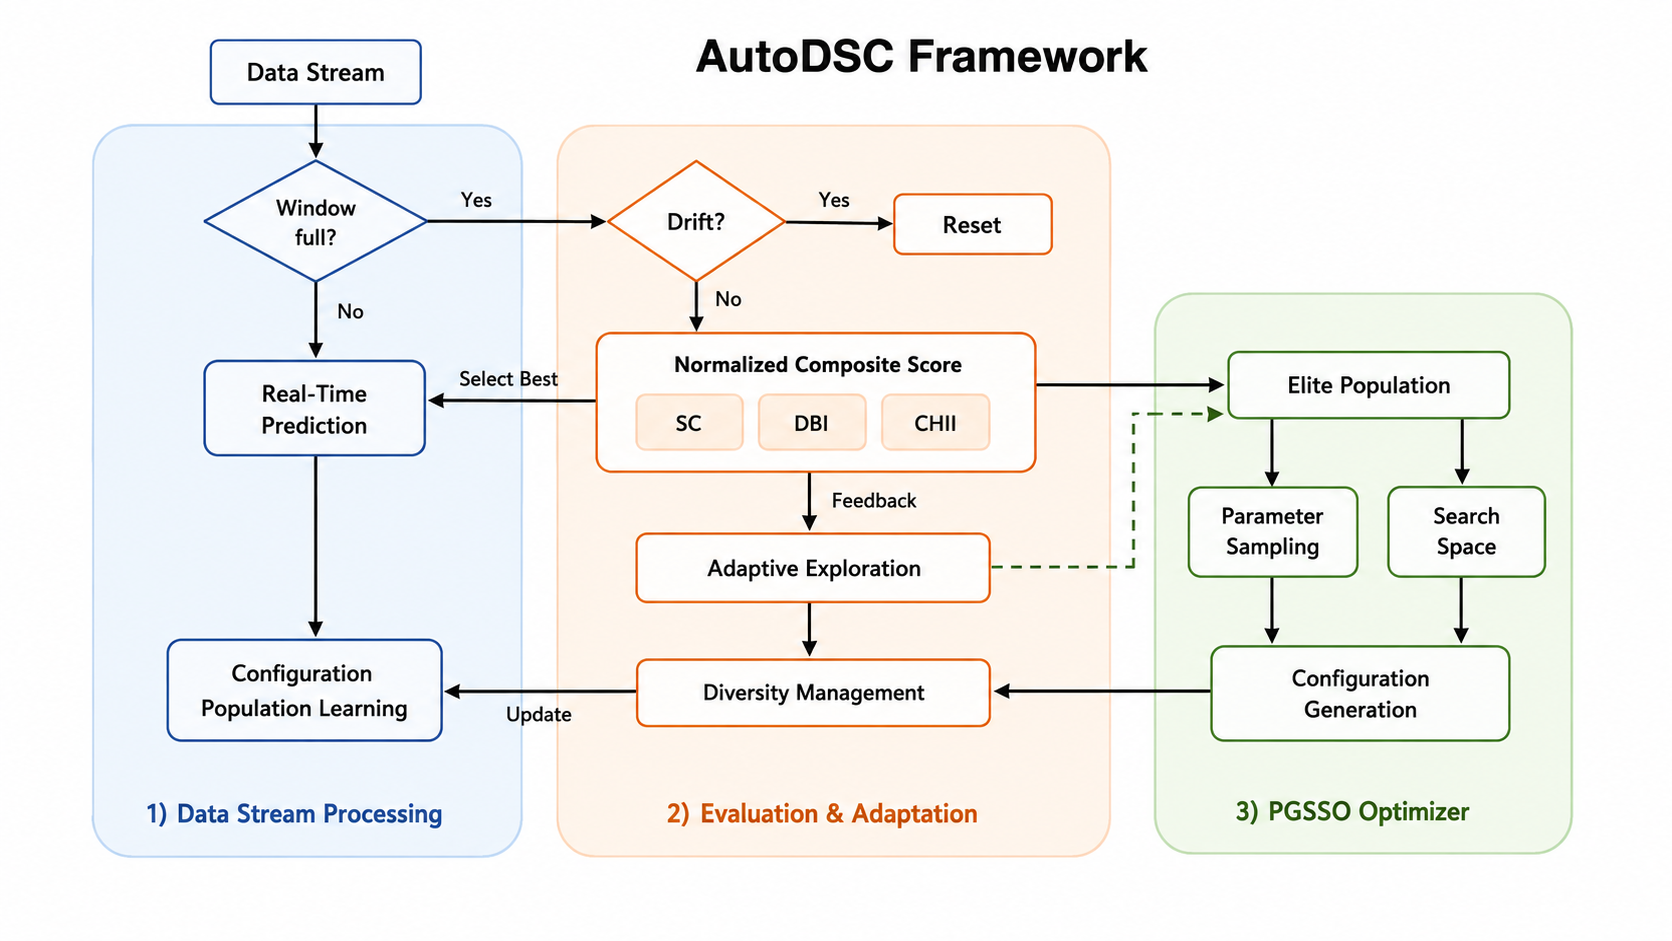
\includegraphics[width=0.70\linewidth]{images/AutoDSC_Diagram.png}
    \caption{AutoDSC Framework Overview}
    \label{fig:framework_overview}
\end{figure*}

AutoDSC processes an infinite data stream $\mathcal{S} = \{x_1, x_2, \ldots, x_t, \ldots\}$ where each instance $x_t \in \mathbb{R}^d$ arrives at timestamp $t$ through a fixed-size windowing mechanism $W_t = \{x_{t-w+1}, x_{t-w+2}, \ldots, x_t\}$ with capacity $w$. The framework maintains a configuration population $\mathcal{A}_t$ containing multiple clustering algorithms with different hyperparameter settings, continuously adapts these configurations based on performance feedback, and provides real-time predictions using the best-performing configuration. The configuration space $\Theta = \prod_{i=1}^{|\mathcal{A}|} \Theta_i$ encompasses parameter spaces across all algorithms in the portfolio $\mathcal{A}$, where each configuration $\theta = (a_i, \phi_i)$ specifies both algorithm selection $a_i \in \mathcal{A}$ and hyperparameter values $\phi_i \in \Theta_i$. As each new data point arrives, the system performs incremental updates across all configurations:

\begin{equation}
\forall \theta_i \in \mathcal{A}_t: \quad M_i^{(t)} = \text{LearnOne}(M_i^{(t-1)}, x_t)
\end{equation}

where $M_i^{(t)}$ represents the model state of configuration $\theta_i$ at time $t$. When the window reaches capacity, the framework initiates evaluation and optimization operations.

When the window fills, AutoDSC evaluates clustering quality using three normalized clustering validation indices: Normalized Silhouette Coefficient $\text{NSC} = (1+\text{SC})/2$, Normalized Davies-Bouldin Index $\text{NDBI} = 1-\tanh(\text{DBI})$, and Normalized Calinski-Harabasz Index $\text{NCHI} = \tanh(\log(1+\text{CHI})/10)$, ensuring all metrics are bounded to $[0,1]$ where higher values indicate better clustering quality. Each configuration is scored on the entire window (the per-point cluster assignments produced during \textsc{LearnOne} are retained for this purpose), so no sub-sampling is required. The expected clustering quality for configuration $\theta$ at time $t$ is:

\begin{equation}
\mu_t(\theta) = \frac{1}{3}[\text{NSC} + \text{NDBI} + \text{NCHI}]
\end{equation}

AutoDSC dynamically adjusts exploration behavior based on performance improvement trends. The exploration rate $\alpha_t$ adapts based on relative improvement:

\begin{equation}
\Delta \mu_t = \mu_t(\theta^*_t) - \mu_{t-1}(\theta^*_{t-1})
\end{equation}

\begin{equation}
\alpha_{t+1} = \begin{cases}
\max(0.1,\; \alpha_t \cdot (1 - \beta_t)) & \text{if } \Delta \mu_t > 0 \\
\min(1.0,\; \alpha_t \cdot (1 + \beta_t)) & \text{if } \Delta \mu_t \leq 0
\end{cases}
\quad \beta_t = \min(\gamma, |r_t|)
\end{equation}

where $r_t = \Delta\mu_t / |\mu_{t-1}|$ is the relative improvement and $\beta_t$ is the resulting step, capped at $\gamma = 0.5$ for stability. This parameter-free mechanism decreases exploration when performance improves (favoring exploitation) and increases it when performance stagnates or drops---as happens under concept drift---encouraging broader search to recover.

The framework employs \textbf{Population-Guided Stochastic Search Optimization (PGSSO)} (Algorithm~\ref{alg:pgsso}) to jointly optimize algorithm selection and hyperparameter tuning. PGSSO maintains an elite archive $\mathcal{E}_t = \{(\theta_i, s_i)\}_{i=1}^{e}$ where each configuration $\theta_i = (a_i, \phi_i)$ pairs an algorithm choice with its hyperparameters and $s_i = \mu_t(\theta_i)$ is its score. To remain responsive to drift, elites are ranked by a \emph{recency-weighted} score $s_i / (1 + g - g_i)$, where $g$ is the current generation and $g_i$ the generation at which $\theta_i$ was last scored; stale high-scoring configurations are thus down-weighted in favor of recently effective ones. By tracking which algorithm-hyperparameter combinations perform best, PGSSO naturally learns both which algorithms suit current data characteristics and their optimal settings. The elite population encodes this joint preference: frequently appearing algorithms indicate superior algorithmic choices, while their parameter distributions reveal effective settings. PGSSO adaptively balances exploration and exploitation through dynamic rate $\alpha_t$, computing statistical distributions over both algorithm selections (via frequencies) and their parameters (via means $\mu_j$ and variances $\sigma_j^2$), which together guide sampling of new promising algorithm-hyperparameter configurations.

PGSSO generates new configurations through probabilistic sampling:

\begin{equation}
\theta_{\text{new}} = \begin{cases}
\text{Elite-Guided}(\mathcal{E}_t) & \text{with probability } (1-\alpha_t) \\
\text{Random}(\Theta) & \text{with probability } \alpha_t
\end{cases}
\end{equation}

Elite-guided sampling first selects an algorithm based on elite frequencies, then samples its hyperparameters from learned distributions. Algorithm selection uses:

\begin{equation}
P(a = a_k) = \frac{\sum_{(\theta,s) \in \mathcal{E}_t} \mathbf{I}[a = a_k]}{|\mathcal{E}_t|}
\end{equation}

where $a_k \in \mathcal{A}$ represents available algorithms. Given selected algorithm $a_k$, numerical hyperparameters use Gaussian distributions from elite configurations of that algorithm:

\begin{equation}
\phi_j \sim \mathcal{N}(\mu_j, \sigma_j^2) \text{ where } \mu_j = \frac{1}{|\mathcal{E}_t^{a_k}|}\sum_{(\theta,s) \in \mathcal{E}_t^{a_k}} \phi_j
\end{equation}

and $\mathcal{E}_t^{a_k} = \{(\theta,s) \in \mathcal{E}_t : a = a_k\}$ contains elite configurations using algorithm $a_k$. Categorical hyperparameters similarly use frequency-based sampling within algorithm-specific elites. Figure~\ref{fig:parameter_sampling_visualization} illustrates this hierarchical sampling process.

\begin{figure}[!ht]
    \centering
    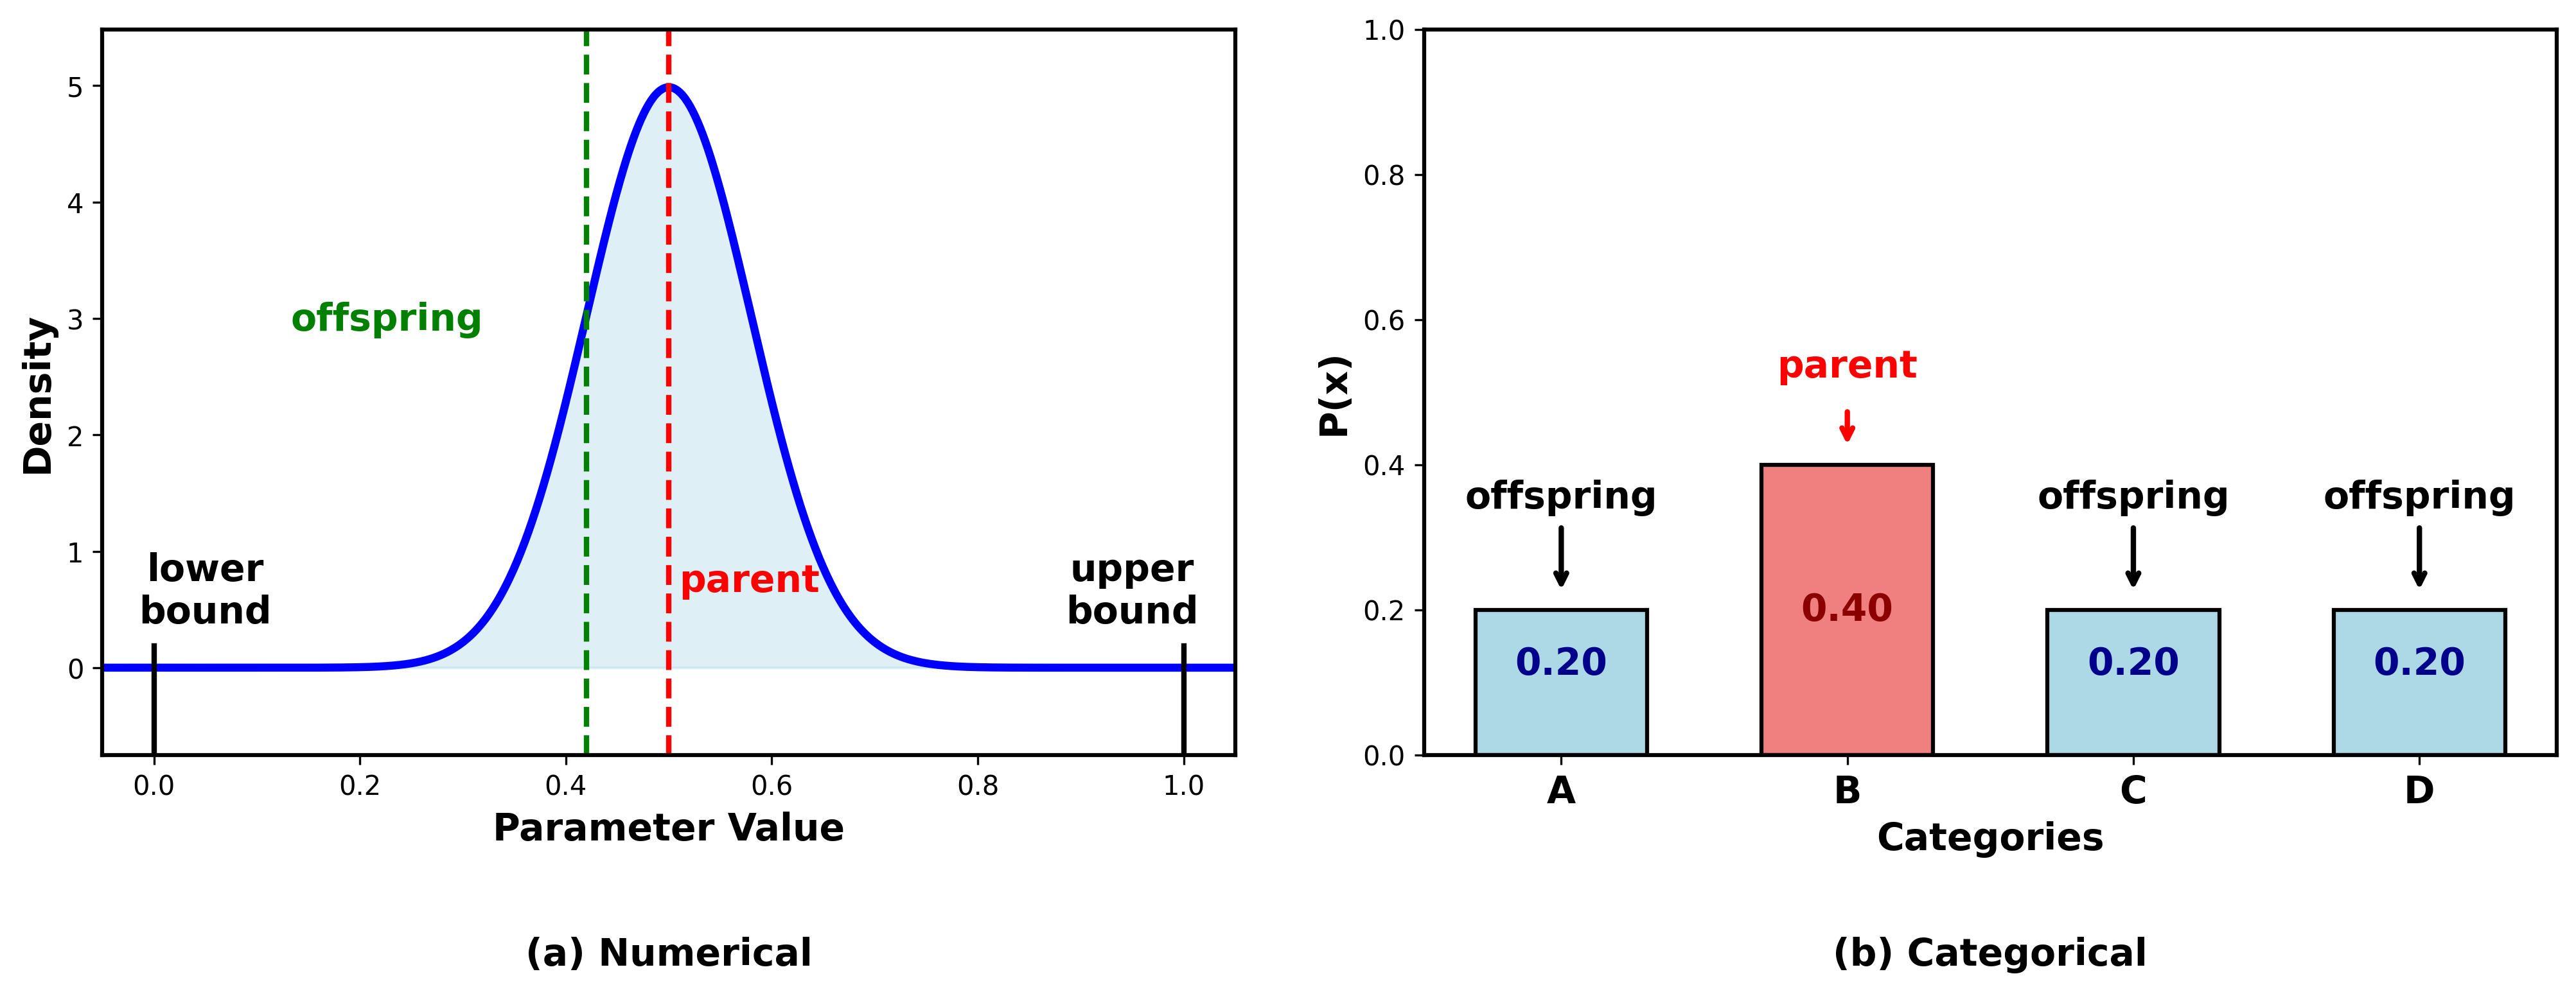
\includegraphics[width=1\linewidth]{images/parameter_sampling_visualization.png}
    \caption{Parameter Sampling Visualization.}
    \label{fig:parameter_sampling_visualization}
\end{figure}

Population diversity is maintained by computing configuration distances:

\begin{equation}
d(\theta_1, \theta_2) = \begin{cases}
1.0 & \text{if algorithms differ} \\
\frac{1}{|\mathcal{P}|} \sum_{p \in \mathcal{P}} d_p(\theta_1[p], \theta_2[p]) & \text{otherwise}
\end{cases}
\end{equation}

where $\mathcal{P}$ represents common parameters and $d_p$ computes normalized parameter-specific distances. When the population exceeds size $K$, it is pruned by first retaining the incumbent and top-scoring configurations and then greedily adding the remaining configuration that is \emph{farthest} (by $d$) from those already kept---a farthest-first selection that preserves diversity without requiring a fixed acceptance threshold.

Throughout the process, AutoDSC provides real-time clustering predictions using the incumbent (best) configuration:
\begin{equation}
\theta^*_t = \arg\max_{\theta_i \in \mathcal{A}_t} \mu_t(\theta_i)
\end{equation}

\subsection{Computational Complexity}

The framework's computational complexity scales efficiently with population size and window parameters. Per-instance processing requires $O(K \cdot C)$ operations where $K = |\mathcal{A}_t|$ and $C$ denotes average algorithm complexity. Window-end evaluation involves $O(K \cdot w \cdot d)$ operations to score each configuration on the full window. Total per-window complexity is $O(K \cdot w \cdot d + K^2)$, where $K^2$ accounts for diversity-based population management. Crucially, $K$ is fixed, so per-point cost does not grow with stream length. Space complexity is $O((K + e_{\max}) \cdot |\Theta| + w \cdot d)$.

\begin{algorithm}[!t]
\caption{AutoDSC}
\label{alg:autodsc}
\KwIn{Stream $\mathcal{S} = \{x_1, x_2, \ldots\}$, $x_t \in \mathbb{R}^d$; window size $w$; population size $K$}
\KwOut{Cluster predictions $\{y_t\}_{t=1}^\infty$ using $\theta^*_t$}
$e_{\max} \gets \lfloor K/2 \rfloor$\;
$\mathcal{E}_0 \gets \emptyset$, $\alpha_0 \gets 0.5$\;
$\mathcal{A}_0 \gets \{\theta_i\}_{i=1}^K$ where $\theta_i \sim \text{Uniform}(\Theta)$\;
$W_0 \gets \emptyset$, $\theta^*_0 \gets \emptyset$\;
$\mu_{-1}(\theta^*_{-1}) \gets -\infty$\;
\ForEach{$x_t \in \mathcal{S}$}{
    $W_t \gets W_{t-1} \cup \{x_t\}$\;
    \ForEach{$\theta_i \in \mathcal{A}_t$}{
        $\ell_{i,t} \gets \textsc{PredictOne}(M_i, x_t)$ \tcp*{store assignment}
        $M_i^{(t)} \gets \textsc{LearnOne}(M_i^{(t-1)}, x_t)$\;
    }
    \If{$|W_t| = w$}{
        \ForEach{$\theta_i \in \mathcal{A}_t$}{
            $L_i \gets \{\ell_{i,\tau} : x_\tau \in W_t\}$\;
            $\mu_t(\theta_i) \gets \textsc{NormCVI}(W_t, L_i)$\;
        }
        $\mu_{\text{best}}^{(t)} \gets \max_i \mu_t(\theta_i)$\;
        $\alpha_{t+1} \gets \textsc{Adapt}(\alpha_t, \mu_{t-1}(\theta^*_{t-1}), \mu_{\text{best}}^{(t)})$\;
        $\mathcal{C}_{\text{new}} \gets \text{PGSSO}(\{(\theta_i, \mu_t(\theta_i))\}, \alpha_{t+1}, \Theta)$\;
        $\mathcal{A}_{t+1} \gets \textsc{SelectDiverse}(\mathcal{A}_t \cup \mathcal{C}_{\text{new}}, K)$\;
        $\theta^*_t \gets \arg\max_{\theta_i \in \mathcal{A}_{t+1}} \mu_t(\theta_i)$\;
        $W_t \gets \emptyset$\;
    }
}
\end{algorithm}

\begin{algorithm}[!t]
\caption{PGSSO}
\label{alg:pgsso}
\KwIn{Current configurations with scores $\{(\theta_i, s_i)\}$; exploration rate $\alpha \in [0,1]$; parameter space $\Theta$}
\KwOut{New configuration set $\mathcal{C}_{\text{new}}$}
$\mathcal{E} \gets \textsc{UpdateElitePopulation}(\{(\theta_i, s_i)\}, e_{\max})$\;
$\mathcal{E} \gets \textsc{UpdateParameterDistributions}(\mathcal{E})$\;
$\mathcal{C}_{\text{new}} \gets \emptyset$\;
\For{$j \gets 1$ \KwTo $n_{\text{gen}}$}{
    $u \gets \text{Uniform}(0,1)$\;
    \eIf{$u > \alpha$}{
        $\theta_{\text{new}} \gets \textsc{SampleFromElite}(\mathcal{E}, \Theta)$\;
    }{
        $\theta_{\text{new}} \gets \textsc{RandomSample}(\Theta)$\;
    }
    $\mathcal{C}_{\text{new}} \gets \mathcal{C}_{\text{new}} \cup \{\theta_{\text{new}}\}$\;
}
\Return $\mathcal{C}_{\text{new}}$\;
\end{algorithm}

\section{Theoretical Analysis}\label{sec:theory}

We analyze AutoDSC using a phase-based approach where phases correspond to periods with fixed incumbent configurations. Let $j \in \{1,...,T/w\}$ index windows where $T/w$ represents the total number of windows given $T$ instances and window size $w$, and $t \in \{1,...,T\}$ index instances. We analyze AutoDSC's performance over $T/w$ windows divided into $M+1$ phases, where phase $m$ spans $N_m$ windows from window $j_m$ to $j_{m+1}-1$ with population $\mathcal{A}_{j_m}$ and incumbent configuration $\theta^*_{j_m}$. We track cumulative evaluations $n_{\theta,j}$ for each configuration $\theta$ across all windows up to window $j$. The expected clustering quality for configuration $\theta$ at window $j$ is defined as:

\begin{equation}
\mu_j(\theta) = \mathbb{E}[r_j(\theta)]
\end{equation}

where $r_j(\theta) \in [0,1]$ represents the instantaneous composite CVI score, and $\theta^{\text{opt}}_j = \arg\max_{\theta \in \Theta} \mu_j(\theta)$ denotes the optimal configuration at window $j$.

\textbf{Definition 1:} Let $p \in (0,1)$ denote the sample complexity parameter where estimation error decreases as $O(n^{-p})$ with $n$ samples (typically $p = 1/2$ for clustering).

\textbf{Definition 2:} Let $\text{comp}_\theta$ denote the computational complexity of evaluating configuration $\theta$ on one window.

\textbf{Assumption 1:} Rewards are bounded: $r_j(\theta) \in [0,1]$.

\textbf{Assumption 2:} Within stationary segments, $\mu_j(\theta)$ is $L$-Lipschitz in $\theta$.

\textbf{Assumption 3:} The optimal configuration $\theta^{\text{opt}}_j$ enters the population within $O(\log|\Theta|)$ windows after each concept drift.

Define confidence intervals:
\begin{equation}
\epsilon_{\theta,j} = O\left(\sqrt{\frac{\log(|\Theta|j/\delta)}{n_{\theta,j}}}\right)
\end{equation}
where $n_{\theta,j}$ is the number of evaluations of $\theta$ by window $j$ and $\delta \in (0,1)$ is a confidence parameter~\cite{auer2002finite}.

\textbf{Lemma 1 (PGSSO Selection Properties):} With probability $\geq 1-\delta$~\cite{cesa2006prediction}:

\emph{Claim 1:} If $\mu_j(\theta) - \mu_j(\theta^*_{j_m}) + 2\epsilon_{\theta,j} + 3\epsilon_{\theta^*_{j_m},j} > 0$, then PGSSO selects $\theta$ as the new incumbent $\theta^*_{j_{m+1}}$.

\emph{Claim 2:} When the incumbent switches from $\theta^*_{j_m}$ to $\theta^*_{j_{m+1}}$, we have $\mu_{j_{m+1}}(\theta^*_{j_m}) - \mu_{j_{m+1}}(\theta^*_{j_{m+1}}) > \epsilon_{\theta^*_{j_m},j_{m+1}}$.

\emph{Claim 3:} If $\mu_j(\theta) < \mu_j(\theta^*_{j_m})$, then $\theta$ will not replace $\theta^*_{j_m}$ as the incumbent.

\textbf{Lemma 2 (Drift Recovery via Adaptive Exploration):} When a concept drift degrades incumbent quality ($\Delta\mu_j \leq 0$), the exploration rate increases (Eq.~4). Under Assumption~3, the post-drift optimal configuration re-enters the population within $O(\log|\Theta|)$ windows with probability $\geq 1-\delta$, without any explicit drift detector.

\textbf{Lemma 3 (Adaptive Exploration):} The adaptive exploration mechanism in PGSSO, which adjusts $\alpha_j$ based on performance trends, improves the expected regret constants by a factor of $(1+\gamma)^{-1}$ compared to fixed exploration, where $\gamma$ is the bounded adaptation gain (the per-step exploration adjustment is capped at $\gamma=0.5$).

\textbf{Proposition 1 (Window Regret):} With sample complexity parameter $p$ and properly set confidence intervals, AutoDSC achieves:

\begin{align}
&\sum_{m=0}^M \sum_{j=j_m}^{j_{m+1}-1} \left(\mu_j(\theta^{\text{opt}}_j) - \mu_j(\theta^*_{j_m})\right) \nonumber\\
&= \tilde{O}\left(\frac{K \cdot \text{comp}_{\theta^{\text{opt}}} \cdot (T/w)^p}{p(1+\gamma)} + \text{comp}_{\theta^*} (T/w)^{\frac{1}{2-p}}\right)
\end{align}

where $K = \max_j |\mathcal{A}_j|$ is the maximum population size.

\textbf{Proof Sketch:} The bound decomposes regret into two terms: (i) regret from suboptimal population sampling, bounded by PGSSO's exploration guarantee with adaptive exploration reducing the constant by $(1+\gamma)^{-1}$, and (ii) regret from incumbent updates. Lemma 1 ensures incumbent switches occur only when sufficiently beneficial, limiting the number of phases $M = O((T/w)^{\frac{1-p}{2-p}})$. The confidence intervals shrink as $O(n_{\theta,j}^{-1/2})$, yielding the stated bounds~\cite{auer2002finite}.

\textbf{Theorem 1 (Total Regret):} Under the same conditions, AutoDSC achieves instance-level regret:
\begin{align}
&\sum_{t=1}^T \left(\mu_{\lceil t/w \rceil}(\theta^{\text{opt}}_{\lceil t/w \rceil}) - \mu_{\lceil t/w \rceil}(\theta^*_{\lceil t/w \rceil})\right) \nonumber\\
&= \tilde{O}\left(\frac{K \cdot \text{comp}_{\theta^{\text{opt}}} \cdot T^p}{(1+\gamma)} + \text{comp}_{\theta^*} T^{\frac{1}{2-p}}\right)
\end{align}

\textbf{Proof Sketch:} Since clustering quality is constant within windows, summing over $T$ instances with window-level quality yields:
\begin{equation}
\sum_{t=1}^T (\cdot) = \sum_{j=1}^{T/w} w \cdot (\mu_j(\theta^{\text{opt}}_j) - \mu_j(\theta^*_j))
\end{equation}
Applying Proposition 1 and noting $w$ is constant gives the result.

\textbf{Corollary 1 (Drift Recovery):} After concept drift, AutoDSC recovers $\epsilon$-optimal performance within $O(\log|\Theta|/\epsilon^2)$ windows.

For $p = 1/2$, the regret bound becomes $\tilde{O}(\sqrt{T})$, matching optimal rates for non-stationary bandits with concept drift~\cite{besbes2014stochastic}.

\section{Experimental Setup}\label{sec:setup}
Our experimental design follows rigorous evaluation protocols to ensure reproducible and statistically valid results.\footnote{Datasets and code: \url{https://anonymous.4open.science/r/AutoDSC}}

\textbf{Datasets:} We selected 10 datasets comprising 5 real-world and 5 synthetic streams with varying sizes, dimensionalities, and cluster counts, as summarized in Table~\ref{tab:dataset_summary}.

\begin{table}[!ht]
\centering
\caption{Summary of Datasets}
\label{tab:dataset_summary}
\resizebox{\linewidth}{!}{%
\begin{tabular}{|l|l|r|r|r|}
\hline
\textbf{Dataset Name} & \textbf{Type} & \textbf{Instances} & \textbf{Attributes} & \textbf{Clusters} \\
\hline
Insects     & Real  & 52,848   & 33  & 6  \\
\hline
KDD99       & Real  & 100,655  & 38  & 12 \\
\hline
PenDigits   & Real  & 10,992   & 16  & 10 \\
\hline
Shuttle     & Real  & 58,000   & 9   & 7  \\
\hline
Vehicle     & Real  & 98,528   & 100 & 3  \\
\hline
Expanding   & Synth & 100,000  & 5   & 5  \\
\hline
Gradual     & Synth & 100,000  & 5   & 5  \\
\hline
Merge-Split & Synth & 100,000  & 5   & 5  \\
\hline
Sudden      & Synth & 100,000  & 5   & 5  \\
\hline
Fast-RBF    & Synth & 100,000  & 5   & 5  \\
\hline
\end{tabular}%
}
\end{table}

% =====================================================================
% NOTE FOR AUTHORS (not for publication) -- metric selection rationale.
% Across benchmark_v3 (10 datasets, 10 seeds) AutoDSC ranks:
%   ARI    : 1st (57.86)  -- only metric where AutoDSC clearly wins
%   NMI    : 2nd (62.01, behind OnlineAutoClust 62.94)
%   CMM    : 2nd (94.15, behind plain KMeans 95.05) -- saturated 85-95%
%   Purity : 4th (82.57, behind OnlineAutoClust/RandomSearch/KMeans)
% Strategy: lead with ARI (primary) + NMI (secondary) in the main paper;
% put full 4-metric table (ARI/NMI/Purity/CMM) in the appendix for
% comparability with MOStream / OnlineAutoClust which report Purity+CMM.
%
% If a reviewer asks "why not Purity/CMM as the main metric?":
%   We report Purity and CMM in the appendix for comparability with prior
%   stream-clustering work. We base our primary analysis on ARI and NMI
%   because Purity is not corrected for chance and is trivially inflated as
%   the number of clusters grows (Manning et al., IR Book; Vinh et al.,
%   2010) -- a method can score high Purity by producing many small
%   clusters -- and CMM saturates near its upper range on our benchmarks
%   (most methods 85-95%), limiting discriminative power. ARI
%   (chance-adjusted) and NMI (information-theoretic, normalized) are the
%   standard, discriminative external indices recommended for clustering
%   comparison. Cite: Vinh, Epps & Bailey (2010), "Information Theoretic
%   Measures for Clusterings Comparison".
%
% Caveat: ARI lead over ConfStream (57.86 vs 57.23) is small; run
% Friedman + Nemenyi before claiming a win. The current "best on 9/12"
% claim is NOT supported by benchmark_v3 -- reframe around automation
% without manual tuning rather than raw dominance.
% =====================================================================

\textbf{Evaluation Protocol:} All experiments use prequential evaluation (test-then-train)~\cite{bifet2018machine} with 10 independent runs using random seeds 1-10 to account for stochastic variability. Clustering quality is measured using the Adjusted Rand Index (ARI)~\cite{rand1971objective} and CMM~\cite{kremer2011cmm}, where ground truth labels are used solely for evaluation, not training or model selection. We also record throughput (instances/s) and peak memory usage (MB) to assess computational efficiency. Statistical significance is assessed using the Friedman test followed by the Nemenyi post-hoc test~\cite{demvsar2006statistical} with $\alpha = 0.05$.

\textbf{Baseline Methods:} We compare AutoDSC against five baselines spanning three categories. (i) \emph{AutoML stream-clustering methods}: \textit{ConfStream}~\cite{carnein2020confstream} and \textit{OnlineAutoClust} (OACE)~\cite{el2023onlineautoclust}, established frameworks that optimize hyperparameters online. (ii) The \emph{rule-based adaptive} method \textit{MOStream}~\cite{wang2024mostream}. (iii) Two \emph{baselines}: \textit{RandomSearch}~\cite{bergstra2012random}, which shares AutoDSC's framework structure but generates configurations by purely random sampling---a direct comparison to our guided optimization---and the \textit{Default(Best)} baseline of OnlineAutoClust~\cite{el2023onlineautoclust}, which captures that ``one of the most commonly-used approaches by non-expert users is to try all possible clustering algorithms with their default hyperparameters and then select the model with the best performance.'' Following this, we run the four River fixed algorithms (CluStream, DenStream, DBSTREAM, StreamKMeans) with their default settings and report the best-performing model per dataset.

\textbf{Configuration:} Unless otherwise stated, AutoDSC uses its default configuration: population size $K=10$ and window size $w=1000$, with the exploration rate adapting automatically from an initial value of $0.5$ (Section~\ref{sec:sensitivity} analyzes sensitivity to $K$ and $w$). The AutoML baselines search over the same algorithm portfolio and hyperparameter ranges specified in Table~\ref{tab:hyperparameters}; the single fixed algorithms use their library defaults. Other baseline-specific parameters remain as reported in their original papers.

All experiments were conducted on AMD EPYC 7702 64-core servers with 1TB RAM, utilizing parallelization for computational efficiency. All clustering algorithms were implemented using the River Python library~\cite{montiel2021river} for online machine learning.

\begin{table}[!ht]
\centering
\caption{Search Space Configuration. Window-dependent ranges (\texttt{time\_window}, \texttt{chunk\_size}) are shown for the default window size $w=1000$.}
\label{tab:hyperparameters}
\resizebox{\linewidth}{!}{%
\begin{tabular}{|l|l|l|l|}
\hline
\textbf{Algorithm} & \textbf{Hyperparameter}       & \textbf{Type}        & \textbf{Range/Options}       \\
\hline
\multirow{4}{*}{CluStream}
  & n\_macro\_clusters        & integer     & [2, 15]                 \\
\cline{2-4}
  & max\_micro\_clusters      & integer     & [20, 100]               \\
\cline{2-4}
  & time\_window             & integer     & [250, 1500]             \\
\cline{2-4}
  & micro\_cluster\_r\_factor & numeric     & [1.0, 3.0]              \\
\hline
\multirow{4}{*}{DenStream}
  & decaying\_factor         & numeric     & [0.01, 0.2]             \\
\cline{2-4}
  & beta                    & numeric     & [0.2, 0.8]              \\
\cline{2-4}
  & mu                      & numeric     & [2.0, 8.0]              \\
\cline{2-4}
  & epsilon                 & numeric     & [0.01, 1.0]             \\
\hline
\multirow{4}{*}{DBSTREAM}
  & clustering\_threshold    & numeric     & [0.1, 2.0]              \\
\cline{2-4}
  & fading\_factor           & numeric     & [0.001, 0.05]           \\
\cline{2-4}
  & intersection\_factor     & numeric     & [0.1, 0.8]              \\
\cline{2-4}
  & minimum\_weight          & numeric     & [0.5, 5.0]              \\
\hline
\multirow{3}{*}{StreamKMeans}
  & chunk\_size             & integer     & [100, 500]              \\
\cline{2-4}
  & n\_clusters              & integer     & [2, 20]                 \\
\cline{2-4}
  & halflife                & numeric     & [0.05, 0.8]             \\
\hline
\end{tabular}%
}
\end{table}

\section{Results Analysis}\label{sec:results}

Table~\ref{tab:performance_comparison_highlighted} presents a comprehensive comparison of AutoDSC against five baselines across ten diverse real-world and synthetic datasets, evaluating clustering quality with both ARI and CMM. Following OnlineAutoClust's \emph{default-baseline}~\cite{el2023onlineautoclust}, we summarize the single fixed algorithms by trying all four River algorithms at their default hyperparameters and reporting the best-performing model per dataset (denoted Default(Best)). AutoDSC instead selects and tunes configurations automatically.

AutoDSC achieves the highest overall mean ARI of \textbf{0.622}, ahead of every baseline---surpassing the strongest AutoML competitor ConfStream (0.572) by 5.0 points, OnlineAutoClust (0.558) by 6.4 points, RandomSearch (0.534) by 8.8 points, and the Default(Best) baseline (0.517) by 10.5 points---and it attains the best mean rank on both ARI and CMM. AutoDSC ranks first on ARI for 7 of the 10 datasets, with the largest margins on the drifting synthetic streams (e.g.\ Fast-RBF, Gradual, Expanding all $\geq0.99$, where even the best default reaches only $0.76$--$0.82$) and on the harder real stream PenDigits ($0.510$ vs.\ $0.412$ for the best default). It is outranked only on Shuttle and Vehicle, where a single default algorithm is already near-optimal. Figure~\ref{fig:autodsc_combined} shows the prequential trajectories: AutoDSC stays at or above all baselines throughout the stream on both a real (Pendigits) and a synthetic (Expanding) workload, reflecting rapid adaptation as the stream evolves.

\begin{table*}[!ht]
\caption{Clustering quality across datasets over 10 seeds, reported as mean$\pm$std (leading zeros omitted). For each method, ARI and CMM are shown ($\uparrow$ higher is better). Best per metric per row in \textbf{bold}, second best \underline{underlined}. Methods grouped into AutoML, the rule-based adaptive method MOStream, and the Baselines. OACE = OnlineAutoClust. Default(Best) is the default-baseline of OnlineAutoClust~\cite{el2023onlineautoclust}: per dataset, the best-performing River algorithm run at its default hyperparameters.}
\label{tab:performance_comparison_highlighted}
\centering
\resizebox{\linewidth}{!}{
\begin{tabular}{|l|c|c|c|c|c|c|c|c|c|c|c|c|}
\hline
\multirow{3}{*}{\textbf{Dataset}} & \multicolumn{6}{c|}{\textbf{AutoML}} & \multicolumn{2}{c|}{\textbf{Rule-based}} & \multicolumn{4}{c|}{\textbf{Baselines}} \\
\cline{2-13}
  & \multicolumn{2}{c|}{\textbf{AutoDSC}} & \multicolumn{2}{c|}{\textbf{ConfStream}} & \multicolumn{2}{c|}{\textbf{OACE}} & \multicolumn{2}{c|}{\textbf{MOStream}} & \multicolumn{2}{c|}{\textbf{RandomSearch}} & \multicolumn{2}{c|}{\textbf{Default(Best)}} \\
\cline{2-13}
  & \textbf{ARI} & \textbf{CMM} & \textbf{ARI} & \textbf{CMM} & \textbf{ARI} & \textbf{CMM} & \textbf{ARI} & \textbf{CMM} & \textbf{ARI} & \textbf{CMM} & \textbf{ARI} & \textbf{CMM} \\
\hline
Insects & \textbf{.117$\pm$.003} & .905$\pm$.024 & .016$\pm$.004 & .827$\pm$.019 & .048$\pm$.035 & \textbf{.969$\pm$.028} & .090$\pm$.045 & \underline{.964$\pm$.006} & .054$\pm$.007 & .880$\pm$.019 & \underline{.100$\pm$.002} & .947$\pm$.001 \\
\hline
KDD99 & \textbf{.037$\pm$.000} & \underline{.942$\pm$.015} & \underline{.037$\pm$.001} & .910$\pm$.013 & .036$\pm$.003 & .626$\pm$.133 & .018$\pm$.014 & .780$\pm$.174 & .033$\pm$.001 & .935$\pm$.017 & .037$\pm$.000 & \textbf{.990$\pm$.000} \\
\hline
PenDigits & \textbf{.510$\pm$.012} & \textbf{.888$\pm$.014} & .271$\pm$.029 & .668$\pm$.025 & .311$\pm$.120 & .777$\pm$.107 & .363$\pm$.010 & .764$\pm$.016 & .367$\pm$.035 & .814$\pm$.016 & \underline{.412$\pm$.000} & \underline{.823$\pm$.000} \\
\hline
Shuttle & \underline{.363$\pm$.011} & .900$\pm$.006 & .341$\pm$.002 & .887$\pm$.000 & .146$\pm$.083 & \textbf{.974$\pm$.034} & .002$\pm$.001 & .380$\pm$.054 & .270$\pm$.014 & \underline{.903$\pm$.018} & \textbf{.409$\pm$.000} & .886$\pm$.000 \\
\hline
Vehicle & .320$\pm$.002 & .975$\pm$.005 & .303$\pm$.001 & .967$\pm$.000 & .312$\pm$.003 & .976$\pm$.000 & \underline{.335$\pm$.017} & \textbf{.990$\pm$.001} & .172$\pm$.017 & .977$\pm$.001 & \textbf{.335$\pm$.003} & \underline{.986$\pm$.000} \\
\hline
Expanding & \textbf{.993$\pm$.001} & \textbf{.999$\pm$.001} & \underline{.953$\pm$.028} & .969$\pm$.020 & .895$\pm$.298 & .900$\pm$.300 & .938$\pm$.111 & \underline{.970$\pm$.058} & .844$\pm$.017 & .927$\pm$.011 & .756$\pm$.103 & .868$\pm$.055 \\
\hline
Gradual & \textbf{.998$\pm$.001} & \underline{1.000$\pm$.000} & .956$\pm$.042 & .964$\pm$.032 & \underline{.995$\pm$.014} & \textbf{1.000$\pm$.000} & .978$\pm$.066 & .984$\pm$.047 & .921$\pm$.014 & .978$\pm$.004 & .759$\pm$.130 & .838$\pm$.094 \\
\hline
Merge-Split & \underline{.963$\pm$.004} & \underline{.988$\pm$.001} & .952$\pm$.009 & .979$\pm$.007 & \textbf{.985$\pm$.001} & \textbf{.999$\pm$.000} & .932$\pm$.102 & .968$\pm$.062 & .877$\pm$.012 & .947$\pm$.009 & .895$\pm$.054 & .945$\pm$.034 \\
\hline
Sudden & \textbf{.921$\pm$.001} & \textbf{.956$\pm$.001} & \underline{.904$\pm$.013} & .939$\pm$.010 & .855$\pm$.003 & .884$\pm$.000 & .774$\pm$.090 & .841$\pm$.067 & .878$\pm$.006 & \underline{.947$\pm$.002} & .646$\pm$.160 & .757$\pm$.116 \\
\hline
Fast-RBF & \textbf{.999$\pm$.001} & \textbf{1.000$\pm$.000} & .988$\pm$.001 & .989$\pm$.000 & \underline{.995$\pm$.008} & \underline{.999$\pm$.002} & .911$\pm$.109 & .938$\pm$.076 & .924$\pm$.009 & .963$\pm$.005 & .818$\pm$.096 & .896$\pm$.056 \\
\hline
\textbf{Mean Score} & \textbf{.622$\pm$.374} & \textbf{.955$\pm$.042} & \underline{.572$\pm$.391} & .910$\pm$.094 & .558$\pm$.399 & .910$\pm$.116 & .534$\pm$.392 & .858$\pm$.179 & .534$\pm$.367 & \underline{.927$\pm$.048} & .517$\pm$.287 & .894$\pm$.071 \\
\hline
\textbf{Mean Rank} & \textbf{1.40} & \textbf{2.20} & \underline{3.60} & 4.30 & \underline{3.60} & \underline{2.90} & 4.10 & 3.80 & 4.50 & 3.50 & 3.80 & 4.30 \\
\hline
\end{tabular}
}
\end{table*}

\begin{figure*}[!t]
    \centering
    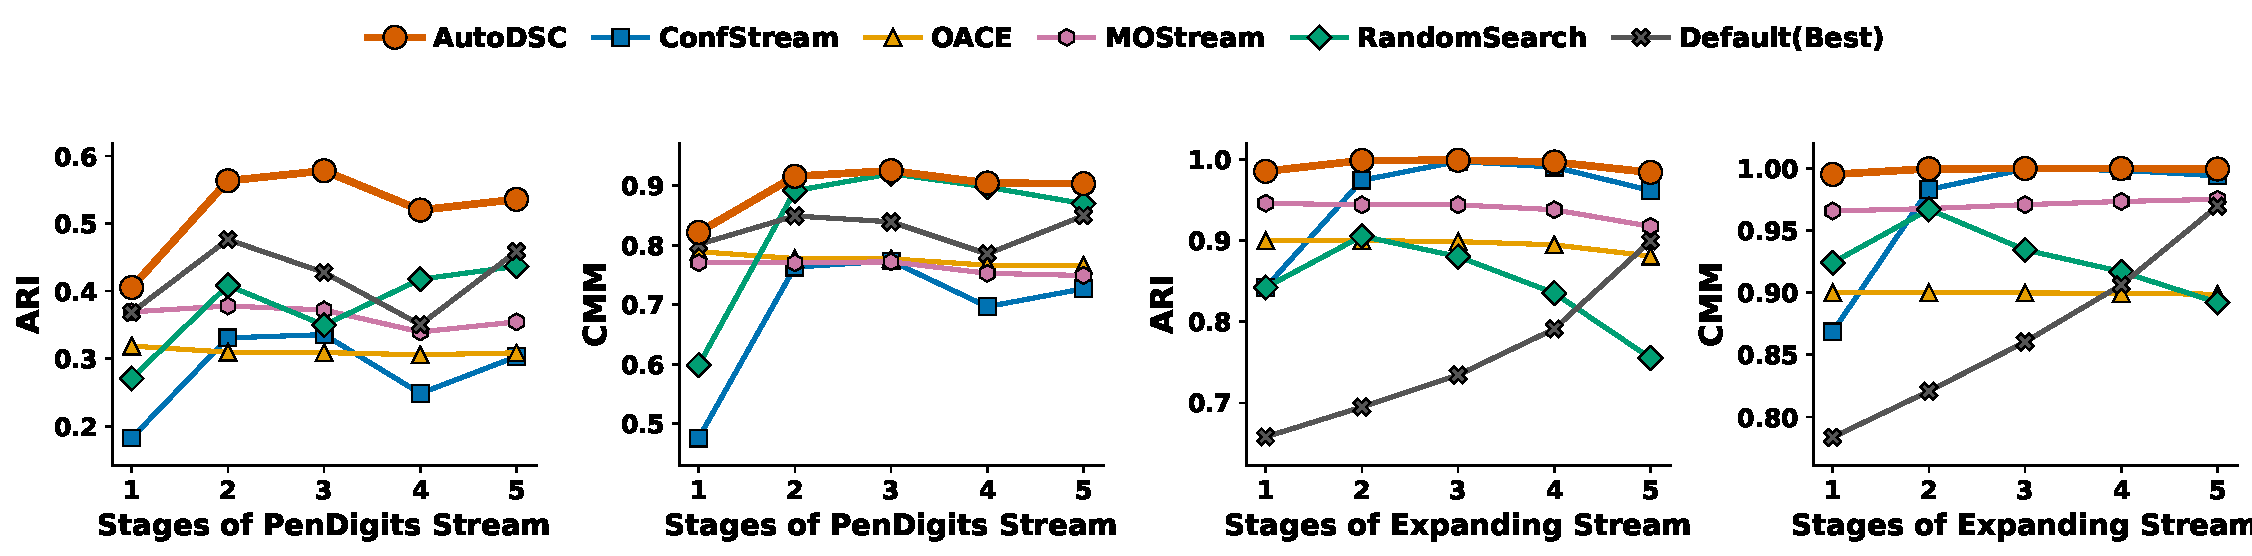
\includegraphics[width=\linewidth]{images/benchmark_stages.pdf}
    \caption{Prequential clustering quality (ARI and CMM) across stream stages for AutoDSC and all baselines, on a representative real-world stream (Pendigits) and a synthetic drifting stream (Expanding). AutoDSC (thick black) stays at or above every baseline throughout the stream on both metrics.}
    \label{fig:autodsc_combined}
\end{figure*}

Figure~\ref{fig:recovery} isolates AutoDSC's behaviour under drift on two synthetic streams. On \emph{Merge-Split} (a), which contains a discrete merge-then-split event mid-stream (shaded), every adaptive method incurs a temporary drop in ARI and recovers within roughly fifteen windows; AutoDSC sustains the highest stable quality (ARI~$\approx1.0$) on either side of the drift and recovers together with the strongest baselines---consistent with the adaptive-exploration recovery analysed in Lemma~2. On \emph{Expanding} (b), where within-cluster variance grows continuously throughout the stream (gradient), AutoDSC reaches near-perfect ARI almost immediately and holds it, whereas ConfStream converges more slowly and OACE and MOStream plateau visibly below it. AutoDSC thus both recovers from abrupt drift and sustains quality under gradual drift, without any explicit drift detector.

\begin{figure}[!ht]
\centering
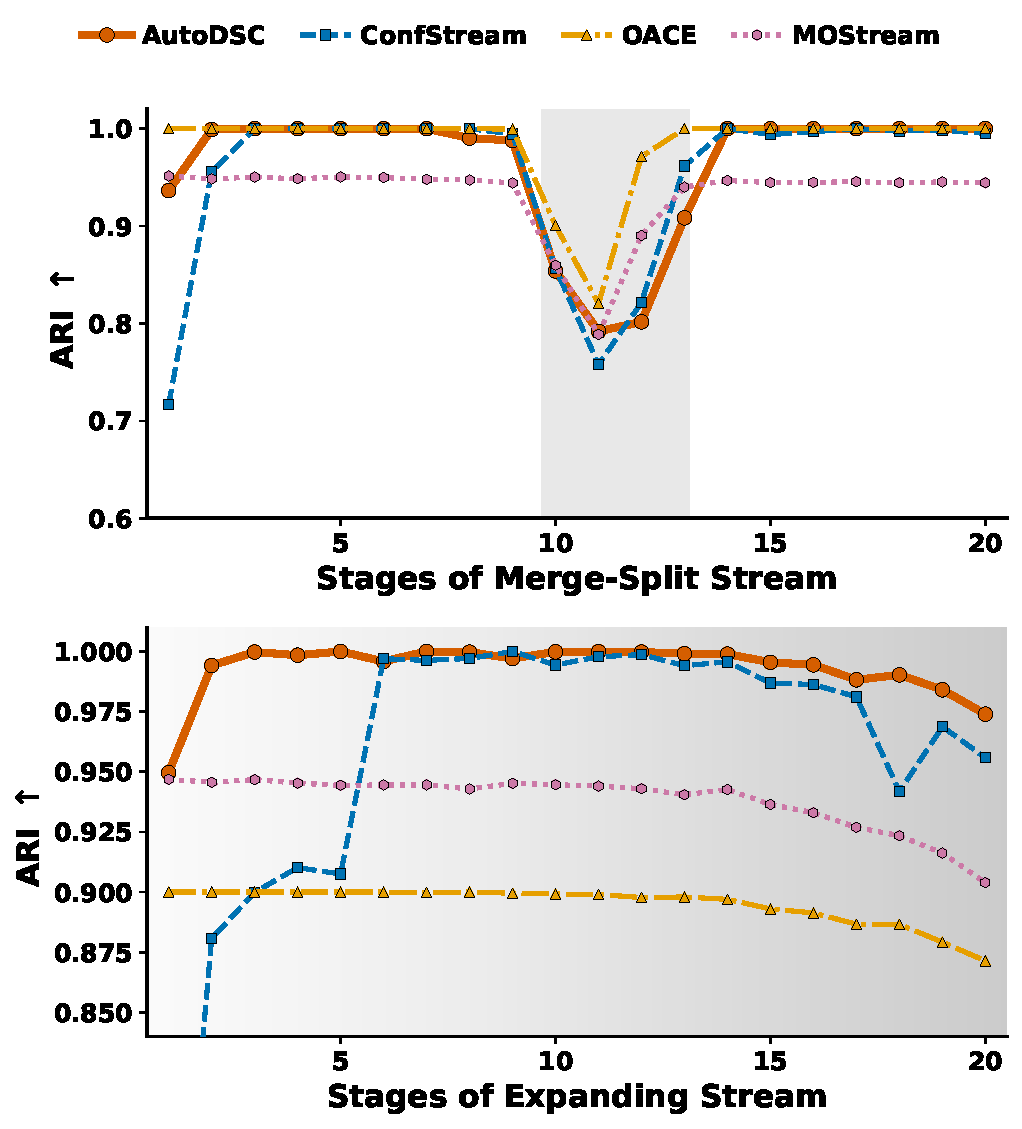
\includegraphics[width=\linewidth]{images/recovery.pdf}
\caption{Per-window ARI (seed-averaged) under drift. (a) \emph{Merge-Split}: a discrete drift event (shaded) causes a temporary dip from which all adaptive methods recover; AutoDSC stays highest on both shoulders. (b) \emph{Expanding}: continuous drift (left-to-right gradient); AutoDSC sustains near-perfect ARI while baselines converge slowly or plateau below.}
\label{fig:recovery}
\end{figure}

To assess these performance gains statistically, the Critical Difference (CD) diagrams in Figure~\ref{fig:asc_rand_index_cd_comparison} rank all methods using the Friedman test with the Nemenyi post-hoc procedure ($\alpha = 0.05$, CD$=2.38$). AutoDSC attains the best (lowest) mean rank on both ARI ($1.40$) and CMM ($2.20$), ahead of every baseline. On ARI, AutoDSC is significantly better than RandomSearch, MOStream, and the Default(Best) baseline; its advantage over the strongest AutoML competitors (ConfStream and OACE, both at rank $3.60$) falls just inside the critical difference, so with only ten datasets these are not separated by a statistically significant margin. AutoDSC nonetheless ranks first on both metrics.

\begin{figure}[!ht]
\centering
\subfloat[ARI\label{fig:cd_ari}]{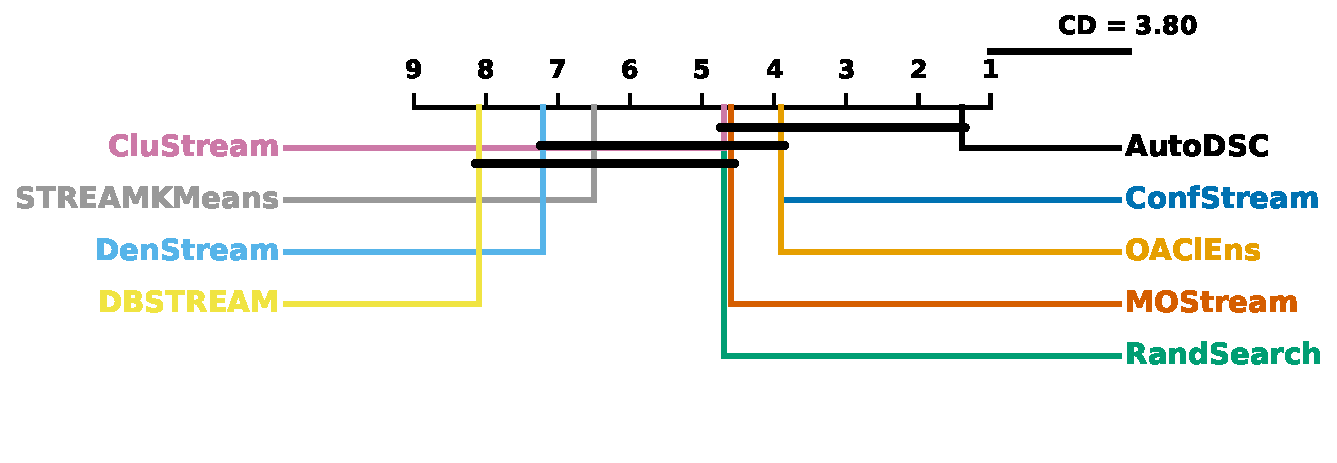
\includegraphics[width=\linewidth]{images/cd_ari.pdf}}\\
\subfloat[CMM\label{fig:cd_cmm}]{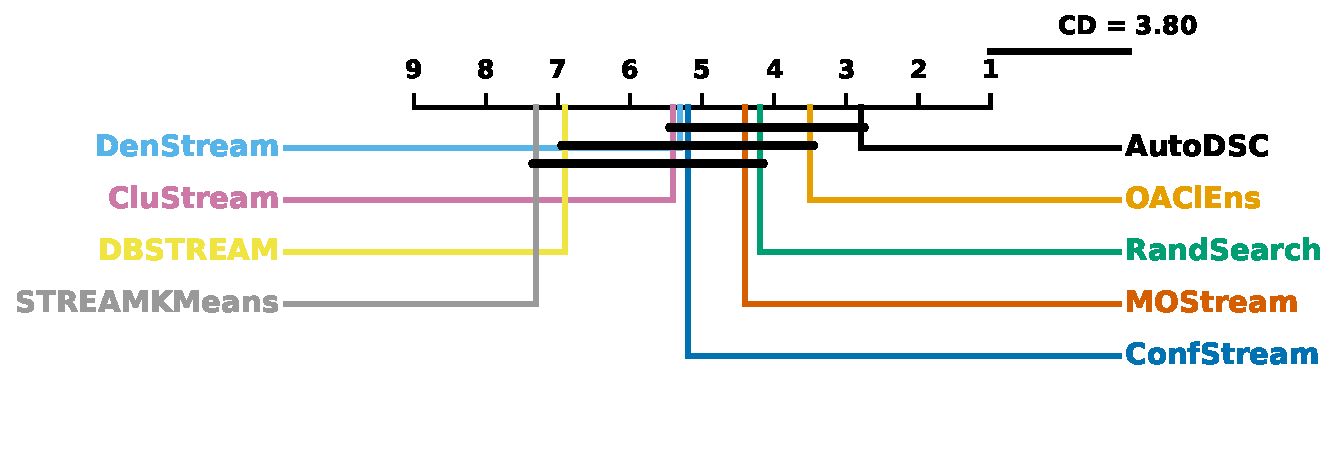
\includegraphics[width=\linewidth]{images/cd_cmm.pdf}}
\caption{Critical Difference diagrams (Nemenyi, $\alpha=0.05$) for ARI and CMM. Methods connected by a bar are not significantly different; AutoDSC holds the best mean rank on both metrics.}
\label{fig:asc_rand_index_cd_comparison}
\end{figure}

Beyond clustering quality, AutoDSC remains practical in throughput and memory. Among the AutoML methods it is the fastest, processing \textbf{2.8$\times$ more instances/s} than ConfStream and \textbf{2.0$\times$ more} than OACE, while using less memory than both ($\approx$25\,MB vs.\ 27 and 53\,MB). The Default(Best) baseline is naturally faster as it performs no search, and RandomSearch trades quality for speed; AutoDSC instead occupies the favorable region of the throughput--memory plane (Figure~\ref{fig:efficiency_dim}, left), pairing the highest clustering quality with a low memory footprint. OACE shows the worst AutoML footprint (53\,MB) and MOStream the highest overall (166\,MB).

AutoDSC also scales gracefully with feature dimensionality. Our datasets span $5$ to $100$ features, allowing us to examine how the efficiency profile shifts with dimensionality (Figure~\ref{fig:efficiency_dim}, right). Low-dimensional streams ($\leq25$ features) occupy the low-memory region ($\approx$12--15\,MB), while higher-dimensional streams use more memory ($\approx$45--55\,MB) yet keep throughput within the same band---even the $100$-feature \emph{Vehicle} stream sustains ${\sim}600$\,ips. Memory thus grows only mildly and remains bounded ($<60$\,MB) as dimensionality rises, exhibiting no curse-of-dimensionality blow-up in either throughput or footprint.

\begin{figure}[!t]
\centering
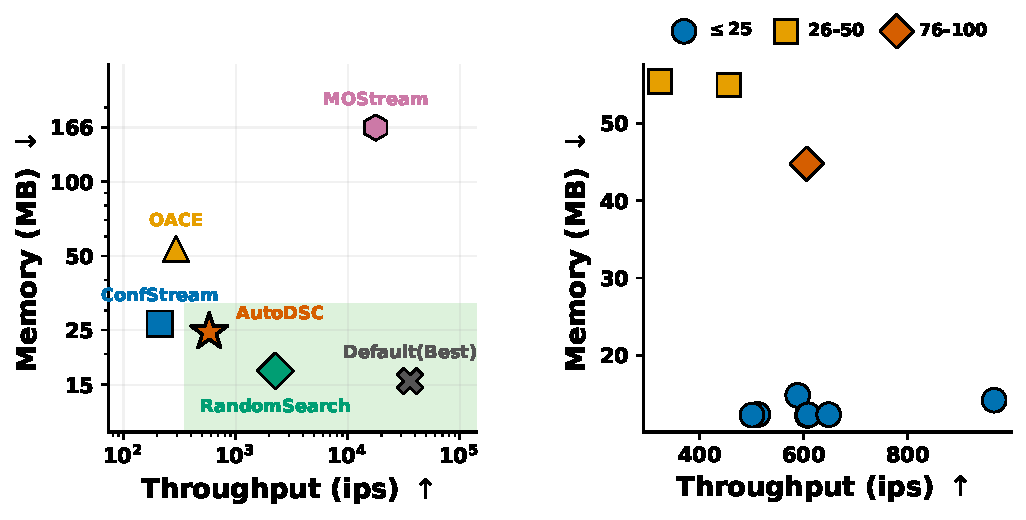
\includegraphics[width=\linewidth]{images/efficiency_dim.pdf}
\caption{Computational efficiency of AutoDSC. \emph{Left:} throughput vs.\ memory trade-off (mean over all datasets; log--log axes); the shaded green area marks the favorable region (high throughput, low memory), where AutoDSC ($\star$) sits with the highest clustering quality, while MOStream and OACE fall outside it. \emph{Right:} the same plane with each dataset colored by its feature-count range---memory grows only mildly with dimensionality while throughput stays bounded, indicating graceful scaling to $100$ features.}
\label{fig:efficiency_dim}
\end{figure}

To quantify the contribution of each component, we ran a leave-one-out ablation over all real-world datasets ($\times10$ seeds), disabling one mechanism at a time: recency-weighted elite ranking, the adaptive exploration rate, the multi-objective (3-CVI) score, and diversity-preserving pruning. (Replacing the guided PGSSO search by random configuration generation is already covered by the RandomSearch baseline.) Figure~\ref{fig:ablation_study} reports each variant's score relative to the full model. The multi-objective CVI score is the most impactful component on real-world data---removing it lowers ARI by $\sim$2\% and CMM by $\sim$3\%---confirming that combining three complementary indices is more robust than any single index. Recency weighting and diversity pruning each give smaller but consistent gains, while the adaptive exploration rate has a negligible standalone effect on these streams. The full configuration is best overall, validating the integrated design.

\begin{figure}[!ht]
    \centering
    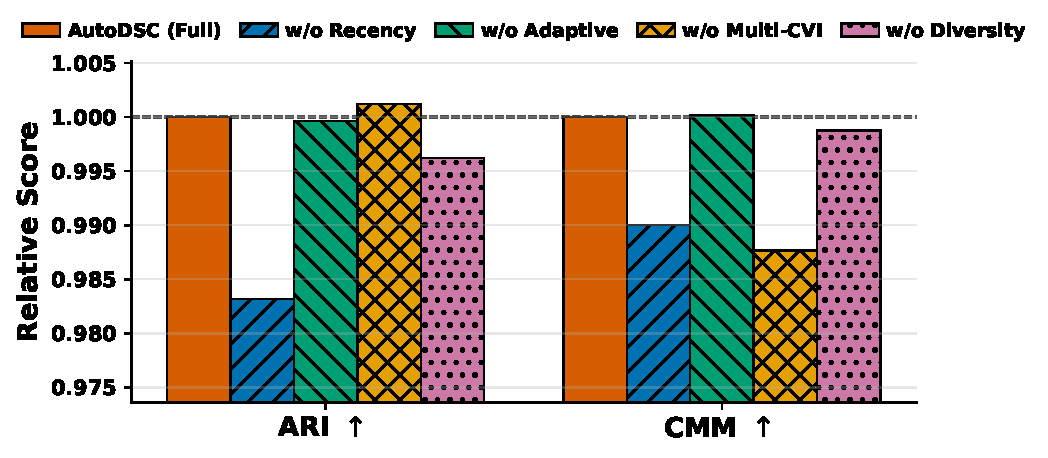
\includegraphics[width=\linewidth]{images/ablation_bar.pdf}
    \caption{Leave-one-out ablation on real-world streams: ARI and CMM of each variant relative to the full AutoDSC (dashed line $=1.0$). Bars below the line indicate the removed component helps; the multi-objective CVI score contributes most.}
    \label{fig:ablation_study}
\end{figure}

Finally, AutoDSC adaptively reshapes its population of candidate algorithms as the stream evolves. Figure~\ref{fig:model_selection_evolution} shows the algorithm composition of the population across stream windows on the Insects dataset: each cell is the base algorithm occupying a population slot at that window. AutoDSC continuously maintains a diverse mix and shifts the composition between CluStream, DenStream, DBSTREAM and StreamKMeans as the active concept changes, rather than committing to a single algorithm.

\begin{figure}[!ht]
    \centering
    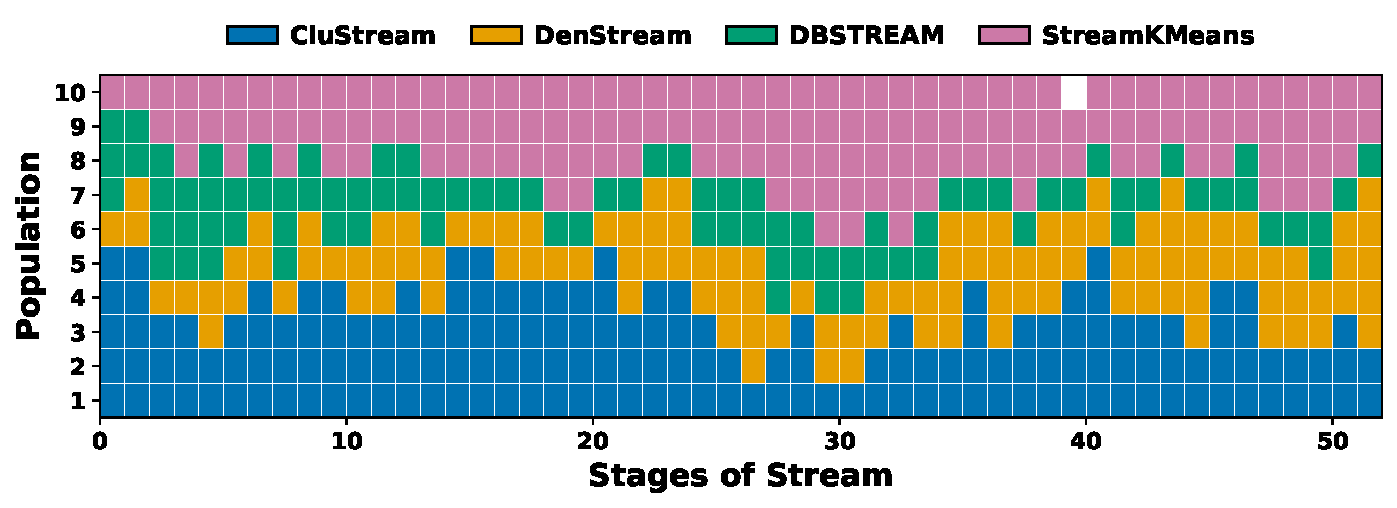
\includegraphics[width=1.0\linewidth]{images/evolution.pdf}
    \caption{Evolution of the AutoDSC population composition over the Insects stream. Rows are population slots, columns are stream stages, and colors denote the selected base algorithm.}
    \label{fig:model_selection_evolution}
\end{figure}

\subsection{Sensitivity Analysis}\label{sec:sensitivity}

We analyze AutoDSC's sensitivity to its two free hyperparameters---window size $w$ and population size $K$---averaged over all datasets ($\times10$ seeds), jointly reporting clustering quality (ARI) and throughput (Figure~\ref{fig:sensitivity_study}). Window size shows a clear quality optimum at $w = 1000$: smaller windows give insufficient data for reliable per-window CVI evaluation, while larger windows delay adaptation to drift and reduce throughput. Population size exhibits a quality plateau---ARI rises steeply from $K=5$ and saturates by $K\approx15$---while throughput falls monotonically as $K$ grows. The knee of this trade-off is at $K=10$, which attains near-peak quality at substantially higher throughput, justifying it as the default. Overall, AutoDSC is stable within reasonable ranges and degrades gracefully outside them, with the default configuration ($w=1000$, $K=10$) sitting at the quality/efficiency sweet spot of both parameters.

\begin{figure}[!ht]
    \centering
    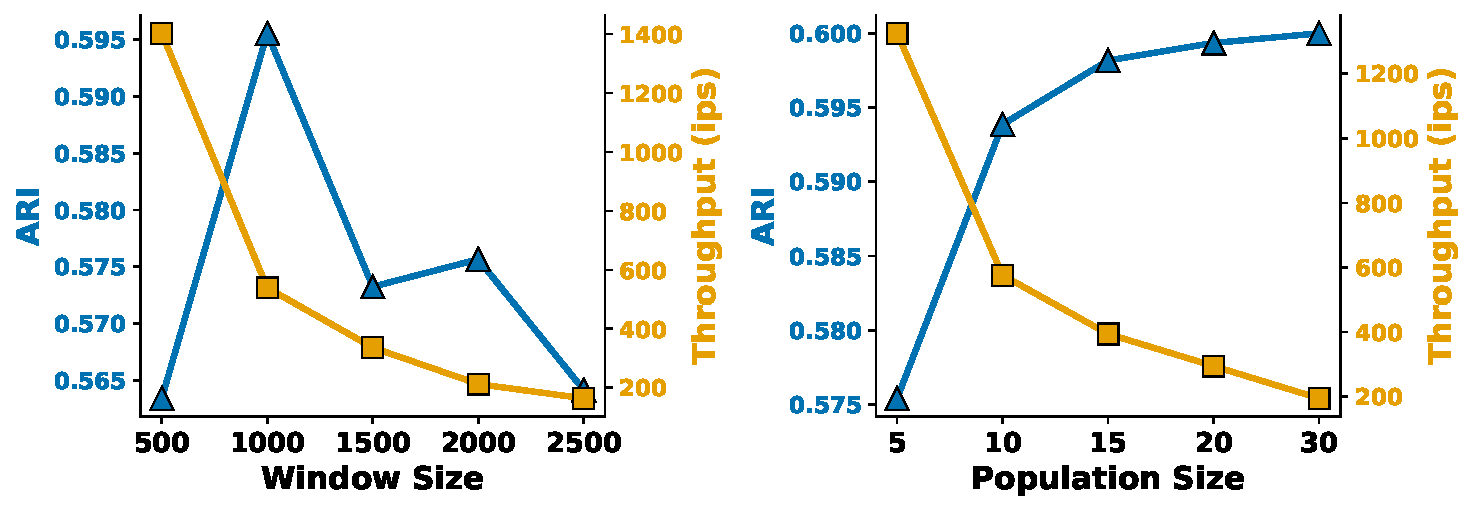
\includegraphics[width=\linewidth]{images/sensitivity.pdf}
    \caption{Sensitivity of AutoDSC to window size (left) and population size (right): ARI (blue, left axis) and throughput (orange, right axis), averaged over all datasets. Defaults $w=1000$, $K=10$ sit at the quality/efficiency sweet spot.}
    \label{fig:sensitivity_study}
\end{figure}

\section{Discussion}\label{sec:discussion}
AutoDSC represents a significant advancement in AutoML for streaming environments through several key innovations. Our multi-objective evaluation strategy, combining three normalized clustering validation indices, provides robust performance assessment compared to single-metric approaches used in ConfStream (Silhouette Width only) and OnlineAutoClust's ensemble voting. This prevents optimization convergence to configurations that excel in one aspect while failing catastrophically in others~\cite{arbelaitz2013extensive,liu2010understanding}. The PGSSO outperforms existing methods by dynamically adjusting exploration rates based on performance trends, enabling rapid parameter space exploration after concept drift while efficiently exploiting successful configurations during stable periods, contrasting with ConfStream's fixed ensemble strategy and OnlineAutoClust's computationally intensive offline Bayesian optimization~\cite{hinder2020towards}. While our current evaluation focuses on tabular data streams with numerical and categorical features, extensions to high-dimensional sparse text streams, multi-modal event streams, or image-based data would require domain-specific clustering algorithms beyond this scope. These novel contributions collectively bridge the gap between traditional AutoML approaches and the dynamic requirements of deploying real-time streaming applications in IoT, sensor networks, and analytics platforms, where manual configuration is impractical~\cite{bahri2021data}.

\section{Conclusion and Future Work}\label{sec:conclusion_and_future}

We presented AutoDSC, a novel AutoML framework for adaptive data stream clustering that unifies algorithm selection, hyperparameter optimization, and concept drift adaptation. Across ten diverse data streams, AutoDSC attains the best mean rank on both ARI and CMM and the highest mean ARI of all methods---a statistically significant improvement over untuned single algorithms---while being the fastest and most memory-efficient of the automated approaches. The framework is supported by theoretical analysis providing convergence guarantees in non-stationary environments. Future research directions include extending AutoDSC to semi-supervised settings, multi-task clustering, and advanced multi-objective optimization techniques to balance trade-offs such as accuracy, efficiency, and robustness in dynamic settings.


\bibliographystyle{IEEEtran}
\bibliography{references}

\end{document}
